\documentclass[reqno]{amsart}
\usepackage[utf8]{inputenc}
\usepackage[margin=1in]{geometry}
\usepackage[usenames, dvipsnames]{xcolor}
\usepackage{graphicx}
\usepackage{mathtools}
\usepackage{amssymb}
\usepackage{amsthm}
\usepackage{fancyhdr}
\usepackage{adforn}
\usepackage{xparse}
\usepackage{tikz}
\usetikzlibrary{fadings}
%\usetikzlibrary{matrix, positioning, calc}
% Additional math macros that I want in both my notes and my psets
\usepackage[sc, noBBpl]{mathpazo}
\usepackage{mathrsfs}
\usepackage[T1]{fontenc}
\usepackage{calligra}
\usepackage{microtype}
\usepackage[all]{xy}
\usepackage{slashed}
\newcommand{\A}{\mathbb A}
\newcommand{\cat}{\mathsf}
\newcommand{\sC}{\cat C}
\newcommand{\sD}{\cat D}
\newcommand{\sS}{\cat S}
\newcommand{\sA}{\mathscr A}
\newcommand{\sF}{\mathscr F}
\newcommand{\sG}{\mathscr G}
\renewcommand{\P}{\mathbb P}
\newcommand{\cO}{\mathscr O}
\newcommand{\sI}{\mathscr I}
\DeclareMathOperator{\coker}{coker}
\renewcommand{\Im}{\operatorname{Im}}
\newcommand{\pt}{\mathrm{pt}}
\DeclareMathOperator{\Hom}{Hom}
\newcommand{\op}{^{\mathsf{op}}}
\newcommand{\Id}{\mathrm{Id}}
\DeclareMathOperator{\Mat}{Mat}
\newcommand{\m}{\mathfrak m}
%\newcommand{\p}{\mathfrak p}
\newcommand{\q}{\mathfrak q}
\DeclareMathOperator{\MSpec}{MSpec}
\DeclareMathOperator{\Spec}{Spec}
\newcommand{\Top}{\cat{Top}}
\newcommand{\Ring}{\cat{Ring}}
\newcommand{\Mod}{\cat{Mod}}
\DeclareMathOperator{\res}{res}
\newcommand{\Alg}{\cat{Alg}}
\newcommand{\Fun}{\cat{Fun}}
\newcommand{\AffSch}{\cat{AffSch}}
\newcommand{\Ab}{\cat{Ab}}
\DeclareMathOperator{\bl}{--}
\DeclareMathOperator{\Free}{Free}
\DeclareMathOperator{\For}{For}
\newcommand{\Set}{\cat{Set}}
\newcommand{\LocRing}{\cat{LocRing}}
\newcommand{\Grp}{\cat{Grp}}
\newcommand{\Sch}{\cat{Sch}}
\newcommand{\inHom}{\operatorname{\underline{\Hom}}}
\DeclareMathOperator{\Frac}{Frac}
\DeclareMathOperator{\Gal}{Gal}
\DeclareMathOperator{\Nil}{Nil}
\newcommand{\pre}{\sC^{\text{pre}}}
\newcommand{\sh}{_{\text{sh}}}
\newcommand{\G}{\mathbb G}
\DeclareMathOperator{\Proj}{Proj}
\newcommand{\sM}{\mathscr M}
\newcommand{\sV}{\mathscr V}
\newcommand{\fU}{\mathfrak U}
\newcommand{\GL}{\mathrm{GL}}
\DeclareMathOperator{\Sym}{Sym}
% http://tex.stackexchange.com/questions/141434/how-to-type-sheaf-hom
\DeclareMathOperator{\shom}{\mathscr{H}\text{\kern -4pt {\calligra\large om}}\,}
\newcommand{\sL}{\mathscr L}
\DeclareMathOperator{\QC}{QC}
\DeclareMathOperator{\Supp}{Supp}
\newcommand{\sN}{\mathscr N}
\DeclareMathOperator{\Ann}{Ann}
\DeclareMathOperator{\Der}{Der}
\newcommand{\ctcpx}[1]{(#1)^{\text{der}}}
\newcommand{\Dist}{\mathsf{Dist}}
\newcommand{\shdi}{\operatorname{Sh}_{\Dist}}
\DeclareMathOperator{\Sh}{Sh}
\newcommand{\shz}{\mathsf{Sh}_{\text{\rm Zar}}}
\DeclareMathOperator{\Gr}{Gr}
% Source: http://tug.org/pipermail/xy-pic/2001-July/000015.html
\newcommand{\pullbackcorner}[1][dr]{\save*!/#1+1.2pc/#1:(1,-1)@^{|-}\restore}
\newcommand{\pushoutcorner}[1][dr]{\save*!/#1-1.2pc/#1:(-1,1)@^{|-}\restore}
\newcommand{\TDel}{\mathrm{2\Delta}}
\DeclareMathOperator{\Bl}{B\ell}
\newcommand{\cR}{\mathcal R}
\newcommand{\cL}{\mathcal L}
\newcommand{\cH}{\mathcal H}
\newcommand{\refR}{\reflectbox{\(\cR\)}}

\renewcommand{\a}{\alpha}
\renewcommand{\b}{\beta}
%\newcommand{\e}{\epsilon}
\renewcommand{\l}{\lambda}
\renewcommand{\L}{\Lambda}
\newcommand{\g}{\gamma}
\newcommand{\s}{\sigma}
\newcommand{\z}{\zeta}
\newcommand{\RR}{\mathbb{R}}
\newcommand{\NN}{\mathbb{N}}
\newcommand{\QQ}{\mathbb{Q}}
\newcommand{\ZZ}{\mathbb{Z}}
\newcommand{\CC}{\mathbb{C}}
\newcommand{\cC}{\mathcal{C}}
\newcommand{\f}{\frac}
\newcommand{\p}{\partial}
\renewcommand{\P}[3][]{\f{\partial^{#1} #2}{\partial #3 ^{#1}}}
%\newcommand{\avg}[1]{\langle #1 \rangle}
\newcommand{\avg}[1]{\left< #1 \right>}
\newcommand{\?}{\overset{?}{=}}
\newcommand{\Int}{\int_{-\infty}^\infty}
\newcommand{\ket}[1]{\left| #1 \right>} % for Dirac bras
\newcommand{\bra}[1]{\left< #1 \right|} % for Dirac kets
\newcommand{\braket}[2]{\left< #1 \vphantom{#2} \right|
 \left. #2 \vphantom{#1} \right>} % for Dirac brackets
\newcommand{\pv}{\vec{p}}

\newcommand{\grad}[1]{\gv{\nabla} #1} % for gradient
\let\divsymb=\div % rename builtin command \div to \divsymb
\renewcommand{\div}[1]{\gv{\nabla} \cdot #1} % for divergence
\newcommand{\curl}[1]{\gv{\nabla} \times #1} % for curl
\renewcommand{\labelenumi}{(\alph{enumi})}
\let\vaccent=\v % rename builtin command \v{} to \vaccent{}
\renewcommand{\v}[1]{\ensuremath{\mathbf{#1}}}
\newcommand{\uv}[1]{\ensuremath{\mathbf{\hat{#1}}}} % for unit vector
\newcommand{\gv}[1]{\ensuremath{\mbox{\boldmath$ #1 $}}} 
% for vectors of Greek letters
\usepackage{hyperref}
\usepackage{siunitx}

%\usepackage[compat=1.1.0]{tikz-feynman}

% TODO fiddle with colors
\definecolor{newblue}{HTML}{1F98A6}
\definecolor{newred}{HTML}{D95448}
\definecolor{neworange}{HTML}{F29441}
\hypersetup{
	colorlinks,
	linkcolor=newred,
	citecolor=neworange,
	urlcolor=newblue!80!black,
}
\usepackage[all]{hypcap}
\pagestyle{plain}
\setcounter{tocdepth}{1}


\usepackage{titlesec}
\titleformat{\section}[frame]
  {\normalfont}
  {\filright
   \footnotesize
   \enspace Lecture \arabic{section}.\enspace}
  {8pt}
  {\Large\bfseries\filcenter}
\usepackage[dotinlabels]{titletoc}
\titlecontents{section}[1.5em]{}{\contentslabel{2.3em}}{\hspace*{-2.3em}}{\hfill\contentspage}

\renewcommand{\sectionmark}[1]{\markleft\thesection. #1}

\fancyhf{}
\fancyhead[RO,LE]{\small\thepage}
\fancyhead[LO]{\small\slshape\nouppercase{\rightmark}}
\fancyhead[RE]{\small\slshape Advanced Quantum Field Theory Lecture Notes}
\setlength{\headheight}{11.0pt}
\pagestyle{fancy}

\numberwithin{equation}{section}
\newcommand{\orbreak}{
\begin{center}
	\adforn{17}\;\(\cdot\)\;\adforn{18}
	\vspace{0.2cm}
\end{center}
}

\renewcommand{\labelitemi}{\(\circ\)}

% I wanted to allow one to reference parts of a thm/cor/etc. and have it print the thm number too, e.g. 29.2(1),
% but this isn't working right now. Probably the best way to do this would be to play around with enumitem to
% define a new enumerate-like counter and then just use that directly instead of enumerate in comp.

% This feels really wobbly, but so far it's working
\NewDocumentEnvironment{comp}{mm}{%
	\csname #1\endcsname\hfill
	\csname #2\endcsname
}{
	\csname end#2\endcsname
	\csname end#1\endcsname
}

% usage:
% \shortexact[f][g]{A}{B}{C},
%
%			 f    g
% for 0 -> A -> B -> C -> 0,
\DeclareDocumentCommand{\shortexact}{O{} O{} mmmm}{
\xymatrix{
	0\ar[r] & #3\ar[r]^-{#1} & #4\ar[r]^-{#2} & #5\ar[r] & 0#6
}}
% exactly the same, but for 0 -> A -> B -> C
\DeclareDocumentCommand{\leftexact}{O{} O{} mmmm}{
\xymatrix{
	0\ar[r] & #3\ar[r]^-{#1} & #4\ar[r]^-{#2} & #5 #6
}}
% ... and the same, for A -> B -> C -> 0
\DeclareDocumentCommand{\rightexact}{O{} O{} mmmm}{
\xymatrix{
	#3\ar[r]^-{#1} & #4\ar[r]^-{#2} & #5\ar[r] & 0#6
}}



% usage:
% X\dblarrow[r] & Y
%   f
% X => Y
%   g
\DeclareDocumentCommand{\dblarrow}{O{} O{} O{}}{
	\ar@<0.4ex>[#1]^-{#2}\ar@<-0.4ex>[#1]_-{#3}
}
% Note: it would be a useful exercise to figure out how to define this so it can be used as
% \dblarrow[r]^f_g

\everyentry={\displaystyle}

\newcommand{\N}{\mathbb N}
\newcommand{\Z}{\mathbb Z}
\newcommand{\Q}{\mathbb Q}
\newcommand{\R}{\mathbb R}
\newcommand{\C}{\mathbb C}
\newcommand{\F}{\mathbb F}
\newcommand{\vp}{\varphi}
\newcommand{\term}{\emph}
\renewcommand{\vec}[1]{\boldsymbol{\mathbf{#1}}}
\DeclarePairedDelimiter\paren{(}{)}
%\DeclarePairedDelimiter\ang{\langle}{\rangle}
\DeclarePairedDelimiter\abs{\lvert}{\rvert}
\DeclarePairedDelimiter\norm{\lVert}{\rVert}
\DeclarePairedDelimiter\bkt{[}{]}
\DeclarePairedDelimiter\set{\{}{\}}
% Swap paren* and paren, etc., so that the normal version resizes by default.
% Meanwhile, one can use \paren*[\Big]{...} to customize the size easily.
% It would be interesting to wrap this up into a custom \definedelimiter command...
\makeatletter
	\let\oldparen\paren
	\def\paren{\@ifstar{\oldparen}{\oldparen*}}
	\let\oldbkt\bkt
	\def\bkt{\@ifstar{\oldbkt}{\oldbkt*}}
\makeatother
\newcommand{\e}{\varepsilon}
\def\qedsymbol{{\small{\ensuremath{\boxtimes}}}}
\newcommand{\inj}{\hookrightarrow}
\newcommand{\surj}{\twoheadrightarrow}
\DeclareMathOperator{\id}{id}
\newcommand{\ud}{\,\mathrm{d}}
\renewcommand{\d}{\mathrm d}
\newcommand{\dfr}[2]{\frac{\mathrm d #1}{\mathrm d #2}}
\newcommand{\pfr}[2]{\frac{\partial #1}{\partial #2}}

%\catcode`\"=13
%\newcommand{"}[1]{^{(#1)}}
\newtheorem{thm}[equation]{Theorem}
\newtheorem*{thm*}{Theorem}
\newtheorem{lem}[equation]{Lemma}
\newtheorem*{lem*}{Lemma}
\newtheorem{cor}[equation]{Corollary}
\newtheorem{prop}[equation]{Proposition}
\newtheorem{obs}[equation]{Observation}
\theoremstyle{definition}
\newtheorem{ex}[equation]{Exercise}
\newtheorem{exm}[equation]{Example}
\newtheorem{defn}[equation]{Definition}
\newtheorem*{claim}{Claim}
\theoremstyle{remark}
\newtheorem*{rem}{Remark}
\newtheorem*{fct}{Fact}
\newtheorem*{note}{Note}

\begin{document}
\title{Symmetries, Fields, and Particles}
\author{Ian Lim\\ Michaelmas 2018}
\maketitle
{\small\noindent These notes were taken for the \textit{Symmetries, Fields, and Particles} course taught by Nick Dorey at the University of Cambridge as part of the Mathematical Tripos Part III in Michaelmas Term 2018. I live-\TeX ed them using Overleaf, and as such there may be typos; please send questions, comments, complaints, and corrections to 
\href{mailto:itel2@cam.ac.uk?subject=SFP\%20Lecture\%20Notes}{\texttt{itel2@cam.ac.uk}}.\\
Many thanks to Arun Debray for the {\LaTeX} template for these lecture notes: as of the time of writing, you can find him at \url{https://web.ma.utexas.edu/users/a.debray/}.}

\tableofcontents

\section{Symmetries, Fields, and Start-icles: Thursday, October 4, 2018}
	\begin{quote}\textit{$2=\pi=i=-1$ in these lectures.} --a former lecturer of Prof. Allanach's.\end{quote}
To begin with, some logistic points. The notes and much of the course material will be based on \href{http://www.damtp.cam.ac.uk/user/tong/qft/qft.pdf}{David Tong's QFT notes} plus some of Prof. Allanach's on cross-sections and decay rates. See \url{http://www.damtp.cam.ac.uk/user/examples/indexP3.html} and in particular \url{http://www.damtp.cam.ac.uk/user/examples/3P1l.pdf} for the notes on cross-sections. In revising these notes, I'll be cross-referencing the Tong QFT notes as well as my copy of Anthony Zee's \textit{Quantum Field Theory in a Nutshell,} which takes a different pedagogical order in starting from the path integral formalism and introducing second quantization (the approach described here) later. Any good education in QFT requires an understanding of both formalisms, and we'll see the path integral next term in \emph{Advanced Quantum Field Theory}.\footnote{Note that the path integral formulation from \emph{Statistical Field Theory}, also taught this term, is precisely equivalent to the path integral that appears in QFT under the identification of one of the Euclidean dimensions of a statistical field theory with the imaginary time dimension of a QFT. This will be more obvious in hindsight.}

After Tuesday's lecture, we'll be assigned one of four course tutors:
\begin{itemize}
    \item Francesco Careschi, fc435@cam.ac.uk
    \item Muntazir Abidi, sma74
    \item Khim Leong, lkw30
    \item Stefano Vergari, sv408
\end{itemize}
Also, the Saturday, November 24th lecture has been moved to 1 PM Monday 26 November, still in MR2. That's it for logistics for now.

\begin{defn}
A \term{quantum field theory} (QFT) is a field theory with an infinite number of degrees of freedom (d.o.f.). Recall that a field is a function defined at all points in space and time (e.g. air temperature is a scalar field in a room wherever there's air). The states in QFT are in general multi-particle states.
\end{defn}
Special relativity tells us that energy can be converted into mass, and so particles are produced and destroyed in interactions (particle number is in general not conserved). This reveals a conflict between SR and quantum mechanics, where particle number is fixed. Interaction forces in our theory then come from additional structure in the theory, depending on things like
\begin{itemize}
    \item symmetry
    \item locality
    \item ``renormalization group flow.''
\end{itemize}

\begin{defn}
A \term{free QFT} is a QFT that has particles but no interactions. The classic free theory is a relativistic theory with which treats particles as excitations of infinitely many quantized harmonic oscillators.
\end{defn}
Free theories are generally not realistic but they are important, as interacting theories can be built from these with perturbation theory. The fact we can do this means the particle interactions are somehow weak (we say these theories have \term{weak coupling}), but other theories of interest (e.g. the strong force) have strong coupling and cannot be described with perturbation theory.

\subsection*{Units in QFT} In QFT, we usually set $c=\hbar=1$. Since $[c]=[L][T]^{-1}$ and $[\hbar]=[L]^2[M][T]^{-1},$ we find that in natural units, $$[L]=[T]=[M]^{-1}=[E]^{-1}$$ (where the last equality follows from $E=mc^2$ with $c=1$, for example). We often just pick one unit, e.g. an energy scale like \si{\electronvolt}, and describe everything else in terms of powers of that unit. To convert back to metres\footnote{As a USAmerican, I am likely to be bewilderingly inconsistent with regards to using American versus British spellings. Please bear with me.} or seconds, just reinsert the relevant powers of $c$ and $\hbar$.

\begin{exm}
The de Broglie wavelength of a particle is given by $\lambda=\hbar/(mc)$. An electron has mass $m_e\simeq \SI{e6}{\electronvolt}$, so $\lambda_e = \SI{2e-12}{\meter}$.
\end{exm}

If a quantity $x$ has dimension $(mass)^d$, we write $[x]=d$, e.g. $$G=\frac{\hbar c}{M_p^2}\implies [G]=-2.$$  $M_p \approx \SI{e19}{\giga\electronvolt}$ corresponds to the Planck scale, $\lambda_p \sim \SI{e-33}{\centi\meter}$, the length/energy scales where we expect quantum gravitational effects to become relevant. We note that the problems associated with relativising the Schr\"odinger equation are fixed in QFT by particle creation and annihilation.

\subsection*{Classical field theory} Before we do QFT, let's review classical field theory. In classical particle mechanics, we have a finite number of generalized coordinates $q_a(t)$ (where $a$ is a label telling you which coordinate you're talking about), and in general they are a function of time $t$. But in field theory, we instead have continuous fields $\phi_a(\vec{x},t)$, where $a$ labels the field in question and $\vec x$ is no longer a coordinate but a label like $a$.\footnote{See for instance Anthony Zee's \textit{QFT in a Nutshell} to see a more detailed description of how we go from discrete to continuous systems.}

In our classical field theory, there are now an infinite number of degrees of freedom, at least one for each position in space $\vec x$, so position has been demoted from a dynamical variable to a mere label.

\begin{exm}
The classical electromagnetic field is a vector field with components $E_i(x,t), B_i(x,t)$ such that $i,j,k\in \{1,2,3\}$ label spatial directions. In fact, these six fields are derived from four fields (or rather four field components), the four-potential $A_\mu(x,t)=(\phi,\vec{A})$ where $\mu\in\{0,1,2,3\}$.

Then the classical fields are simply related to the four-potential by
\begin{equation}
E_i=\P{A_i}{t}-\P{A_0}{x_i} \text{ and } B_i=\frac{1}{2}\epsilon_{ijk} \P{A_k}{x_j}
\end{equation}
with $\epsilon_{ijk}$ the usual \href{https://en.wikipedia.org/wiki/Levi-Civita_symbol}{Levi-Civita symbol}, and where we have used the Einstein summation convention (repeated indices are summed over).
\end{exm}

The dynamics of a field are given by a \term{Lagrangian} $L$, which is simply a function of $\phi_a(x,t), \dot \phi_a(x,t),$ and $\grad \phi_a(x,t)$. This is in precise analogy to the Lagrangian of a discrete system, which is a function of the coordinates $q_a(t)$ and their derivatives $\dot q_a(t)$.
\begin{defn}
We write
\begin{equation}
L=\int d^3 x \mathcal{L}(\phi_a, \p_\mu \phi_a),
\end{equation}
where we call $\mathcal{L}$ the \term{Lagrangian density}, or by a common abuse of terminology simply the Lagrangian.
\end{defn}
\begin{defn}
We may then also define the \term{action}
\begin{equation}
S\equiv \int_{t_0}^{t_1}L dt = \int d^4x \mathcal{L}(\phi_a,\p_\mu \phi_a)
\end{equation}
\end{defn}
Let us also note that in these units we take the action $S$ to be dimensionless, $[S]=0$ (since it appears alone in an exponent, for instance, $e^{iS}$), and so since $[d^4x]=-4$ we have $[\mathcal{L}]=4.$

The dynamical principle of classical field theory is that fields evolve such that $S$ is stationary with respect to variations of the field that don't affect the initial or final values (boundary conditions). That is, $\delta S=0$. A general variation of the fields produces a variation in the action
$$\delta S=\sum_a \int d^4 x\left \{ \P{\mathcal{L}}{\phi_a}\delta\phi_a +\P{\mathcal{L}}{(\p_\mu\phi_a)} \delta(\p_\mu \phi_a)\right\}.$$
Integrating the second term by parts, we find that the variation in the action becomes
$$\delta S= \sum_a \int d^4x \left\{ \P{\mathcal{L}}{\phi_a}\delta \phi_a +\p_\mu \left( \P{\mathcal{L}}{(\p_\mu \phi_a)}\delta \phi_a\right)-\p_\mu \left(\P{\mathcal{L}}{(\p_\mu \phi_a)}\right)\delta \phi_a\right\}.$$

The integral of the total derivative term vanishes for any term that decays at spatial $\infty$ (i.e. $\mathcal{L}$ is reasonably well-behaved) and has $\delta \phi_a(x,t_1)=\delta \phi_a(x,t_0)=0$, as guaranteed by our boundary conditions. Therefore the boundary term goes away and we find that stationary action, $\delta S=0$, implies the \term{Euler-Lagrange equations},
\begin{equation}
\p_\mu\P{\mathcal{L}}{(\p_\mu\phi_a)}-\P{\mathcal{L}}{\phi_a}=0.
\end{equation}

\begin{exm}
Consider the Klein-Gordon field $\phi$, defined as the real-valued field $\phi$ which has a Lagrangian
\begin{equation}
\mathcal{L}=\frac{1}{2} \eta^{\mu\nu}\p_\mu \phi \p_\nu \phi -\frac{1}{2}m^2 \phi^2.
\end{equation}
Here $\eta^{\mu\nu}$ is the standard Minkowski metric\footnote{We use the mostly minus convention here, but honestly the sign conventions are all arbitrary and relativity often uses the other one where time gets the minus sign.}.

To compute the Euler-Lagrange equation for this field theory,
 we see that $$\P{\cL}{\phi}=-m^2\phi \text{ and } \P{\cL}{(\p_\mu \phi)}=\p^\mu \phi.$$
The Euler-Lagrange equations then tell us that $\phi$ obeys the equation of motion $$\p_\mu \p^\mu \phi+m^2\phi = 0,$$ which we call the \emph{Klein-Gordon equation}. It has wave-like solutions $\phi=e^{-ipx}$ with $(-p^2+m^2)\phi=0$ (so that $p^2=m^2$, which is what we expect in units where $c=1$).
\end{exm}

\subsection*{Non-lectured aside: on functional derivatives} If you're like me, you get a little anxious about taking complicated functional derivatives. The easiest way to manage these is to rewrite the Lagrangian so that all terms precisely match the form of the quantity you are taking the derivative with respect to, and remember that matching indices produce delta functions. 

Here's a quick example. To compute $\P{}{(\p_\alpha \phi)}\left[ \p_\mu \phi \p^\mu \phi\right]$, rewrite the term in the brackets as $\eta^{\mu\nu}\p_\mu \phi \p_\nu \phi$ (since we are deriving with respect to a function of the form $\p_\alpha \phi$) and make sure to take the derivative with respect to a new index not already in the expression, e.g. $\p_\alpha \phi$. Then 
\begin{eqnarray*}
\P{}{(\p_\alpha \phi)}\left[ \p_\mu \phi \p^\mu \phi\right]&=&\P{}{(\p_\alpha \phi)}\eta^{\mu\nu}\p_\mu \phi \p_\nu \phi\\
&=& \eta^{\mu\nu} (\delta^\alpha_\mu)\p_\nu \phi + \eta^{\mu\nu} \p_\mu \phi (\delta _\nu^\alpha)\\
&=&2\p^\alpha \phi,
\end{eqnarray*}
where we have raised the index with $\eta^{\mu\nu}$ and written the final expression in terms of $\alpha$ using the delta function. The functional derivative effectively finds all appearances of the denominator exactly as written, including indices up or down, and replaces them with delta functions so the actual indices match. This is especially important in computing the Euler-Lagrange equations for something like Maxwell theory, where one may have to derive by $\p_\mu A_\nu$ and both those indices must match exactly to their corresponding appearances in the Lagrangian.

No one ever taught me exactly how to approach such variational problems, so I wanted to record my strategy here for posterity. It may take a little longer than just recognizing that $\P{}{(\p_\mu \phi)} \frac{1}{2}\p_\nu \phi \p^\nu \phi = \p^\mu \phi$, but this approach always works and it has the benefit of helping avoid careless mistakes like forgetting the factor of $2$ in the example above.
\section{Symmetry Described Simp-Lie: Saturday, October 6, 2018}
	Last time, we derived the Euler-Lagrange equations for Lagrangian densities:
\begin{equation}
\p_\mu \P{\mathcal{L}}{(\p_\mu \phi_a)}-\P{\mathcal{L}}{\phi_a}=0.
\end{equation}
Today, we'll look at some more simple Lagrangians. We'll introduce Noether's theorem as it applies to fields and also derive the energy-momentum tensor in a field theory context.

\begin{exm}
Consider the Maxwell Lagrangian,
\begin{equation}
\mathcal{L}=-\frac{1}{2}(\p_\mu A_\nu)(\p^\mu A^\nu)+\frac{1}{2}(\p_\mu A^\mu)^2.
\end{equation}
Plugging into the E-L equations, we find that $\P{\cL}{A_\nu}=0$ and
\begin{equation}
\P{\cL}{(\p_\mu A_\nu)}=\p^\mu A^\nu +\eta^{\mu\nu}\p_\rho A^\rho.
\end{equation}
Thus E-L tells us that
\begin{equation}
0=-\p^2 A^\nu+\p^\nu (\p_\rho A^\rho)=-\p_\mu(\p^\mu A^\nu-\p^\nu A^\mu).
\end{equation}
Defining the field strength tensor $F^{\mu\nu}=\p^\mu A^\nu-\p^\nu A^\mu$, we can write the E-L equation for Maxwell as the simple
$$0=\p_\mu F^{\mu\nu},$$
which written explicitly is equivalent to Maxwell's equations in vacuum (we'll revisit this when we do QED).
\end{exm}

The Lagrangians we'll consider here and afterwards are all \term{local}-- in other words, there are no couplings $\phi(\vec{x},t)\phi(\vec{y},t)$ with $\vec{x}\neq \vec{y}$. There's no reason a priori that our Lagrangians have to take this form, but all physical Lagrangians seem to do so.

\subsection*{Lorentz invariance} Consider the Lorentz transformation on a scalar field $\phi(x)\equiv \phi (x^\mu)$. The coordinates $x$ transform as $x'=\Lambda^{-1} x$ with $\Lambda^\mu{}_\sigma \eta^{\sigma\tau}\Lambda^\nu{}_\tau = \eta^{\mu\nu}$. Under $\Lambda,$ our field transforms as $\phi\to \phi'$ where $\phi'(x)=\phi(x')$. Recall that Lorentz transformations generically include boosts as well as rotations in $\RR^3$. As we've discussed in Symmetries, Fields and Particles, Lorentz transformations form a Lie group ($O(3,1)$, or specifically the proper orthochronous Lorentz group) under matrix multipication. They have a representation given on the fields (i.e. a mapping to a set of transformations on the fields which respects the group multiplication law).

For a scalar field, this is $\phi(x)\to \phi(\Lambda^{-1}x)$ (an active transformation). We could have also used a passive transformation where we re-label spacetime points: $\phi(x)\to \phi(\Lambda x)$. It doesn't matter too much-- since Lorentz transformations form a group, if $\Lambda$ is a Lorentz transformation, so is $\Lambda^{-1}$. In addition, most of our theories will be well-behaved and Lorentz invariant.

\begin{defn}
\term{Lorentz invariant} theories are ones where the action $S$ is unchanged by Lorentz transformations.
\end{defn}

\begin{exm}
Consider the action given by
$$S=\int d^4x \left[\frac{1}{2} \p_\mu \phi \p^\mu \phi-U(\phi)\right],$$
where $U(\phi)$ is some potential density. $U\to U'(x) \equiv U(\phi'(x))= U(x')$ means that $U$ is a scalar field (check this!) and we see that
$$\p_\mu \phi' =\P{}{{x^\mu}}\phi(x')=\P{{{x'}^\sigma}}{{x^\mu}} \p_\sigma' \phi(x')= (\Lambda^{-1})^\sigma{}_\mu \p_\sigma' \phi(x')$$
where $\p_\sigma' \equiv \P{}{{{x'}^\sigma}}$.
Thus the kinetic term transforms as
$$\cL_{kin} \to \cL_{kin}'=\eta^{\mu\nu}\p_\mu \phi' \p_\nu \phi' =\eta^{\mu\nu}(\Lambda^{-1})^\sigma{}_\mu (\Lambda^{-1})^\tau{}_\nu \p_\sigma' \phi(x') \p_\tau' \phi(x')=\eta^{\sigma\tau} \p_\sigma' \phi(x')\p_\tau' \phi(x') = L_{kin}(x).$$

Thus we see that the action overall transforms as
$$S\to S' = \int d^4 x \cL(x')=\int d^4 x \cL(\Lambda^{-1}x).$$
Under a change of variables $u \equiv \Lambda^{-1} x$, we see that $\det(\Lambda^{-1})=1$ (from group theory) so the volume element is the same, $d^4y=d^4x$ and therefore
$$S'=\int d^4 y\, \cL(y)=S.$$
We conclude that $S$ is invariant under Lorentz transformations.
\end{exm}

We also remark that under a LT, a vector field $A_\mu$ transforms like $\p_\mu \phi$, so $$A_\mu'(x) = (\Lambda^{-1})^\sigma{}_\mu A_\sigma (\Lambda^{-1}x).$$
This is enough to attempt Q1 from example sheet 1.\footnote{Copied here for quick reference: Show directly that if $\phi(x)$ satisfies the Klein-Gordon equation, then $\phi(\Lambda^{-1} x)$ also satisfies this equation for any Lorentz transformation $\Lambda.$}

\begin{thm}
Every continuous symmetry of $\cL$ gives rise to a current $J^\mu$ which is conserved, $\p_\mu j^\mu=0$. Each $j^\mu$ has a conserved charge $Q=\int_{\RR^3} j^0 d^3x$.
\end{thm}
Given that the current is conserved, it's easy to show that the charge is conserved, since $\frac{dQ}{dt}=\int_{\RR^3} d^3x \p_0 j^0  = -\int_{\RR^3} d^3 x \div {\vec{j}} =0$ by the divergence theorem, assuming $|\vec{j}|\to 0$ as $|\vec{x}|\to \infty$.

Let us define an infinitesimal variation of a field $\phi$,
$\phi(x)\to \phi'(x)=\phi(x)+\alpha \Delta \phi(x)$
with $\alpha$ an infinitesimal change. If $S$ is invariant, we call this a \term{symmetry} of the theory.

Since $S$ is invariant up to adding a total 4-divergence (a total derivative $\p_\mu$) to the Lagrangian, our symmetry doesn't affect the Euler-Lagrange equations. $\cL$ transforms as
\begin{equation}\label{lagrangeinfinitesimal}
    \cL(x)\to \cL(x)+\alpha \p_\mu X^\mu(x),
\end{equation}
and expanding to leading order in $\alpha$ we have
\begin{equation}
    \cL\to \cL(x)+\alpha \P{\cL}{\phi}\Delta \phi +\alpha \P{\cL}{(\p_\mu\phi)}\p_\mu(\Delta\phi)+O(\alpha^2).
\end{equation}
We can rewrite this in terms of a total derivative $\p_\mu\left(\P{\cL}{(\p_\mu\phi)}\Delta \phi\right)$
so that
\begin{equation}
\cL'=\cL(x)+\alpha \p_\mu\left(\P{\cL}{(\p_\mu\phi)}\Delta \phi\right) +\alpha \left(\P{\cL}{\phi}-\p_\mu \P{\cL}{(\p_\mu\phi)}\right)\Delta \phi.
\end{equation}
By Euler-Lagrange, the second term in parentheses vanishes, so we identify the first term in parentheses as none other than $\alpha \p_\mu X^\mu(x)$ from Eqn. \ref{lagrangeinfinitesimal} (in other words, $\p_\mu\left(\P{L}{(\p_\mu\phi)}\Delta \phi\right) =\p_\mu X^\mu$) and recognize 
\begin{equation}
j^\mu\equiv\P{L}{(\p_\mu \phi)}\Delta \phi -X^\mu
\end{equation} as our conserved current (such that $\p_\mu j^\mu =0$).

\begin{exm}
Take a complex scalar field $$\psi(x)=\frac{1}{\sqrt{2}}(\phi_1(x)+i\phi_2(x)).$$ We can then treat $\psi, \psi^*$ as independent variables and write a Lagrangian
$$L=\p_\mu \psi^* \p^\mu \psi - V(|\psi|^2).$$
Then we observe that under $\psi\to e^{i\beta}\psi, \psi^* \to e^{-i\beta}\psi^*,$ the Lagrangian is invariant. The differential changes are $\Delta \psi = i \psi$ (think of expanding $\psi\ \to e^{i\beta}\psi$ to leading order) and similarly $\Delta \psi^*=-i\psi^*$ (here we find that $X^\mu=0$).

We add the currents from $\psi, \psi^*$ to find
$$j^\mu = i\set{ \psi \p_\mu \psi^* - \psi^* \p_\mu \psi}.$$
\end{exm}
This is enough to do questions 2 and 3 on the example sheet.
\begin{exm}
Under infinitesimal translation $x^\mu \to x^\mu -\alpha \epsilon^\mu$, we have $\phi(x)\to \phi(x)+\alpha \epsilon^\mu \p_\mu \phi(x)$ by Taylor expansion (similar for $\p_\mu\phi$). If the Lagrangian doesn't depend explicitly on $x$, then $\cL(x)\to \cL(x) +\alpha \epsilon^\mu \p_\mu \cL(x)$.

Rewriting to match the form $\cL+\a \p_\mu X^\mu$, we see that our new Lagrangian takes the form
$L(x)+\alpha \epsilon^\nu \p_\mu (\delta^\mu_\nu L)$. We get one conserved current for each component of $\epsilon^\nu$, so that
$$(j^\mu)_\nu = \P{\cL}{(\p_\mu \phi)}\p_\nu \phi - \delta^\mu_\nu \cL$$ with $\p_\mu(j^\mu)_\nu=0$.
We write this as $j^\mu{}_\nu \equiv T^\mu{}_\nu$, the energy-momentum tensor. 

\begin{defn}
The \term{energy-momentum tensor} (sometimes \term{stress-energy tensor}) is the conserved current corresponding to translations in time and space. It takes the form 
$$T^{\mu\nu} \equiv \P{\cL}{(\p_\mu \phi)}\p^\nu \phi - \eta^{\mu\nu} \cL,$$
where we have raised an index with the Minkowski metric as is conventional. The conserved charges from integrating $\int d^3x T^{0\nu}$ end up being the total energy $E=\int d^3x T^{00}$ and the three components of momentum $P^i=\int d^3x T^{0i}$.\footnote{The definition of the energy-momentum tensor here is slightly different from the one used in general relativity. Here, we have used time and space translations to derive $T^{\mu\nu}$, but in general relativity, we use variations of the metric $g^{\mu\nu}$ instead. The benefit of the GR definition is that the resulting tensor is always symmetric, whereas the $T^{\mu\nu}$ from spacetime translations is not guaranteed to be symmetric. We'll see an example of this in the example sheets, but the $T^{\mu\nu}$ defined by spacetime translations can always be \emph{made} symmetric by defining the ``Belinfante-Rosenfeld tensor.'' The construction isn't anything too special, but relativists insist that variations of the action with respect to the metric is the correct way to define the energy-momentum tensor.}
\end{defn}
\end{exm}
\section{Here Comes the $SO(n)$: Tuesday, October 9, 2018}
	Having introduced the matrix groups, we'll next discuss some important subgroups of $GL(n,\RR)$. First, the \term{orthogonal groups.}
\begin{defn}
Orthogonal groups $O(n)$ are the matrix groups which preserve the Euclidean inner product,
\begin{equation}
O(n)=\set{M\in GL(n,\RR): M^T M = I_N}.
\end{equation}
Their elements correspond to orthogonal transformations, so that for $\vec{v}\in \RR^n$, an orthogonal matrix $M$ acts on $\vec{v}$ by matrix multiplication,
$$\vec{v}'=M\cdot \vec{v}$$
and so in particular
$$|\vec{v}'|^2={\vec{v}'}^T \cdot \vec{v}' = \vec{v}^T \cdot M^T M \cdot \vec{v}= \vec{v}^T \cdot \vec{v}=|\vec{v}|^2.$$
It also follows that $\forall M\in O(n), \det(M^TM)=\det(M)^2 = \det(I_n) = 1 \implies \det M =\pm 1$.
\end{defn}
$\det M$ is a smooth function of the coordinates, but our constraint equation means that $\det M$ can only take on one of two discrete values. The orthogonal group $O(n)$ has therefore two connected components corresponding to $\det M = +1$ and $\det M = -1$. The connected component containing the origin ($\det M = +1$) is the special orthogonal group $SO(n)$.
\begin{defn}
The \term{special orthogonal groups} $SO(n)$ are the subset of orthogonal groups which also preserve orientation (i.e. no reflections):
$$SO(n)\equiv \set{M\in O(n): \det M = +1}.$$
That is, elements of $SO(n)$ preserve the sign of the volume element in $\RR^n$,
$$\Omega= \epsilon^{i_1 i_2 \ldots i_n} v_1^{i_1}v_2^{i_2}\ldots v_n^{i_n}.$$
\end{defn}
In contrast, $O(n)$ matrices may include reflections as well as rotations when $\det M = -1$.

\begin{ex}\label{groupaxiomsson}
Check the group axioms for $SO(n)$.\footnote{As usual, we need to check closure and inverses. The identity matrix $I$ satisfies $I^TI=I$ and $\det I=1$, and associativity follows from standard matrix multiplication. Inverses: if $M\in SO(n)$, then $M^{-1}$ is defined by $MM^{-1}=I$. But $\det(MM^{-1})=\det(M)\det(M^{-1})=(1)\det(M^{-1})=\det I = 1$, so $\det(M^{-1})=1$. We also check that the inverse of an orthogonal matrix is also orthogonal: $M M^{-1}=I$, so $(M^{-1})^T (M^T)= (M^{-1})^T M^{-1} =I^T = I$. Closure: $\forall M,N \in SO(n), \det(MN)=\det(M)\det(N)=(1)(1)=1$ and $(MN)^T(MN)=N^TM^T M N= I$, so $MN\in SO(n)$. \qed}
Show that $\dim(O(n))=\dim(SO(n))=\frac{1}{2} n(n-1)$.\footnote{This can be seen by writing a matrix $M\in SO(n)$ as a row of $n$ column vectors $(\vec{x_1},\vec{x_2},\ldots,\vec{x_n})$. Then the condition that $M^T M = 1$ is equivalent to
$\begin{pmatrix}
\vec{x_1}\cdot \vec{x_1} & \vec{x_1}\cdot \vec{x_2} & \ldots &\vec{x_1}\cdot \vec{x_n}\\
\vec{x_2}\cdot \vec{x_1} & \vec{x_2}\cdot \vec{x_2} & \ldots &\vec{x_2}\cdot \vec{x_n}\\
\vdots\\
\vec{x_n}\cdot \vec{x_1}& \ldots & \ldots & \vec{x_n} \cdot \vec{x_n}
\end{pmatrix}= I_n.$
We see that by the symmetry of the explicit form of $M^T M$, we get $1+2+3+\ldots+n = n(n+1)/2$ independent constraints on the $n^2$ entries of $M$. Applying our theorem, we find that the resulting manifold has dimension $n^2-n(n+1)/2=n(n-1)/2$.
} 
\end{ex}

Orthogonal matrices have some nice properties. Let $M \in O(n)$ be an orthogonal matrix and suppose that $\vec{v}_\lambda$ is an eigenvector of $M$ with eigenvalue $\lambda.$ Then the following is true:
\begin{enumerate}
\item If $\lambda$ is an eigenvalue, then $\lambda^*$ is also an eigenvalue (eigenvalues of $M$ come in complex conjugate pairs).
\item $|\lambda|^2=1$.
\end{enumerate}
The proof is as follows:
\begin{enumerate}
\item $M\cdot \vec{v}_\lambda = \lambda \vec{v}_\lambda \implies M\cdot \vec{v}_\lambda^* = \lambda^* \vec{v}_\lambda^*$ (since $M$ is a real matrix).\footnote{This is generally true of real matrices with complex eigenvalues-- it's not specific to orthogonal matrices.}
\item For any complex vector $\vec{v}$, we have
$$(M\cdot \vec{v}^*)^T \cdot M \cdot \vec{v} = \vec{v}^\dagger \cdot M^T M \cdot \vec{v} = \vec{v}^\dagger \cdot \vec{v}.$$ Now if $\vec{v}=\vec{v}_\lambda$, then
$$(M\cdot \vec{v}_\lambda^*)^T \cdot M \cdot \vec{v}_\lambda=(\lambda^* \vec{v}^*_\lambda)^T \cdot (\lambda \vec{v}_\lambda)=|\lambda|^2 \vec{v}_\lambda^\dagger \cdot \vec{v}_\lambda.$$
By comparison to the first expression, we see that $|\lambda|^2=1$. \qed
\end{enumerate}

\begin{exm}
For the group $G=SO(2)$, $M\in SO(2)\implies M$ has eigenvalues
$$\lambda=e^{i\theta},e^{-i\theta}$$ for some $\theta\in\RR,\theta \sim \theta+2\pi$ (identified up to a phase of $2\pi$). A group element may be written explicitly as
$$M=M(\theta)=\begin{pmatrix}
\cos\theta & -\sin\theta\\
\sin\theta & \cos\theta
\end{pmatrix},$$
which is uniquely specified by a rotation angle $\theta$. Therefore the group manifold of $SO(2)$ is $M(SO(2))\cong S^1$, the circle, and we see that $SO(2)$ is an abelian group..

It's not too hard to check using the trig addition formulas that the matrices $M$ written this way really do form a representation of $SO(2)$, since $M(\theta_1) M(\theta_2)=M(\theta_1+\theta_1)$.
\end{exm}
\begin{exm}
For the group $G=SO(3)$, we have instead $M\in SO(3)\implies M$ has eigenvalues
$$\lambda=e^{i\theta},e^{-i\theta},1$$ for $\theta\in \RR,\theta \sim \theta+2\pi$, using our two properties again of paired eigenvalues and modulus 1.
The normalized eigenvector for $\lambda=1$, $\uv n \in \RR^3$, specifies the axis of rotation ($M \cdot \uv n = \uv n$ and $\uv n \cdot \uv n = 0$).

A general group element of $SO(3)$ can be written explicitly as
\begin{equation}
M(\uv n, \theta)_{ij} = \cos\theta\delta_{ij} +(1-\cos\theta)n_i n_j - \sin\theta \epsilon_{ijk} n_k.
\end{equation}
Let us remark that our group is invariant under the identification $\theta\to 2\pi-\theta, \uv n \to -\uv n$. It's also true that we should identify all $M$ with $\theta=0$ since $M(\uv n, 0)= I_3 \forall \uv n$.

We also observe that we can consider the vector
$$\vec{w}\equiv\theta \uv n$$ which lives in the region
$$B_3=\set{\vec{w}\in \RR^3: |\vec w|\leq \pi} \subset \RR^3$$
with boundary
$$\partial B_3 = \set{\vec{w}\in \RR^3: |\vec{w}|=\pi} \cong S^2.$$
We say that the group manifold $M(SO(3))$ then comes from identifying antipodal points on $\p B_3$ ($\vec{w} \sim -\vec{w} \forall \vec{w} \in \p B_3$). See Fig. \ref{so3manifold} for an illustration.
\end{exm}

\begin{figure}\label{so3manifold}
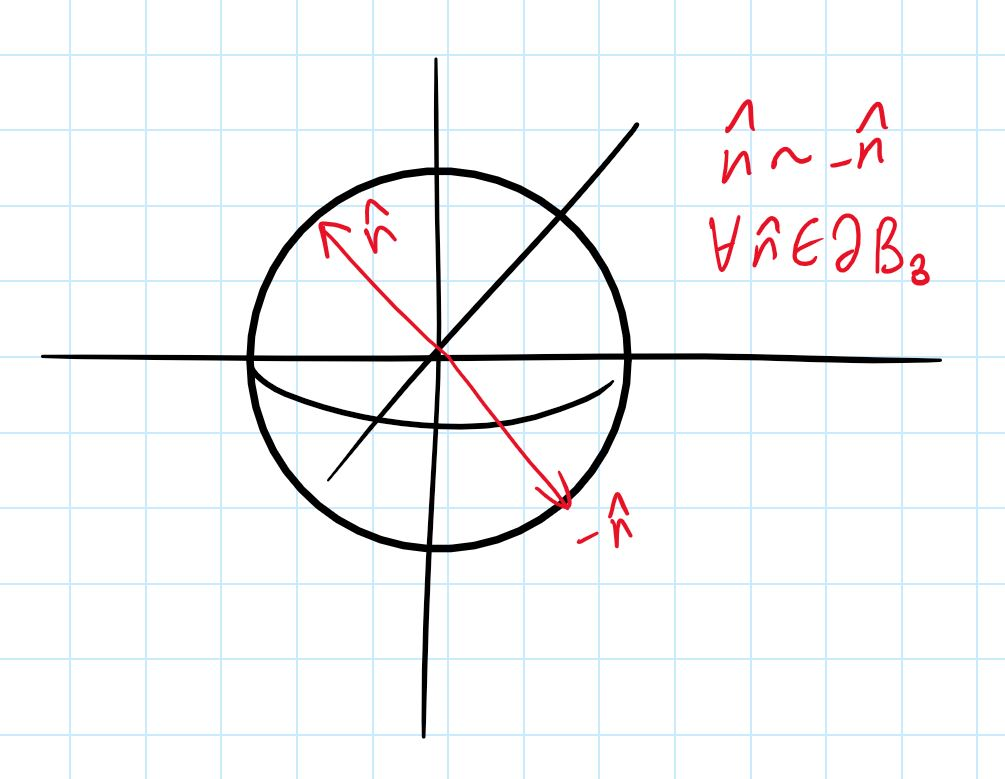
\includegraphics[scale=0.7]{2018/10/20181009_img1}
\caption{The group manifold $M(SO(3))$ is isomorphic to the 3-ball $B^3$ with antipodal points on the boundary identified, $\vec{w} \sim -\vec{w} \forall \vec{w} \in \p B_3$.}
\end{figure}

\begin{defn}
A \term{compact} set is any bounded, closed set in $\RR^n$ with $n\geq 0$. For instance, the $2$-sphere $S^2$ is clearly bounded in $\RR^3$. But the hyperboloid $H^2$ (embedded in $\RR^3$ as $x^2+y^2-z^2 =r^2$) is not bounded, since for any distance $r_0$ one can construct a point $\vec{x}$ on $H^2$ which has $|\vec{x}|>r_0$.
\end{defn}

Let us note some properties of the group manifold $M(SO(3))$. It is compact and connected, but it is not simply connected.
\begin{defn}
A space is \term{simply connected} if all loops on the space are contractible (in the language of algebraic topology, its fundamental group $\pi_1$ is trivial).
\end{defn}
A bit of intuition for why $M(SO(3))$ is topologically non-trivial: draw a path to the boundary, come out on the antipodal side, and go back to the origin. As it turns out, this is different from $S^1$ or the torus $T^2$: whereas these have the full $\ZZ$ as (part of) their fundamental groups ($T^2$ is simply $S^1\times S^1$), if we go around twice in $SO(3)$ we find that this new loop is actually a trivial loop (see Fig. \ref{z2inso3}). Therefore the fundamental group of $SO(3)$ is not infinite but the cyclic group $\ZZ_2$ (i.e. the set $\set{0,1}$ under the group operation $+\mod 2$).

\begin{figure}\label{z2inso3}
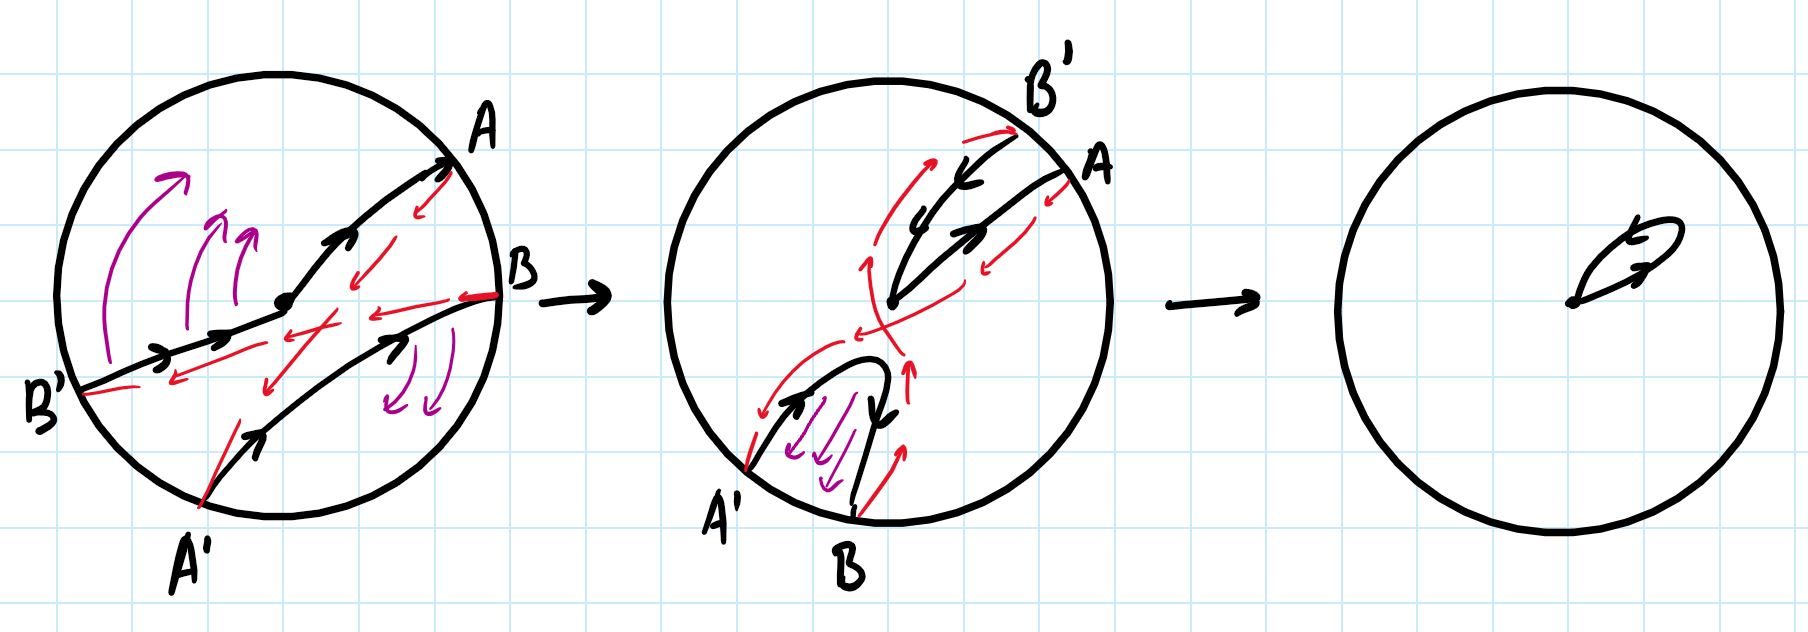
\includegraphics[scale=0.6]{2018/10/20181009_img2}
\caption{A sketch of why the loop which goes through the boundary $\p B_3$ twice is homotopic to (can be continuously deformed into) the trivial loop. For simplicity, consider a circular cross-section of $B_3$ and suppose the loop passes through the boundary at points $A$ ($\sim A'$) and $B$ ($\sim B'$). As we continuously move the point $B$ to $A'$, $B'$ must also move towards $A$, as we see in the second image. We then pull the bit of loop from $A'$ to $B$ through the boundary and find that the resulting loop is trivial (sketch 3). Solid black lines indicate the actual loop path, red dashed arrows indicate the effect of identifying antipodal points, and purple arrows suggest the direction of loop deformation between each drawing.}
\end{figure}
\section{Here Comes the $SU(n)$: Thursday, October 11, 2018}
	Recall that for a free scalar field $$\phi(\vec{x},t)=\int \frac{d^3 \vec{p}}{(2\pi)^3} e^{i \vec{p}\cdot \vec{x}}\phi(\vec{p},t),$$ where
$$\left[\P[2]{}{t}+(\vec{p}^2 +m^2)\right]\phi(\vec{p},t)=0.$$
We also defined $\omega_{\vec{p}}^2\equiv \vec{p}^2 +m^2$.
Our theory has plane wave solutions. 
Let's apply the simple harmonic oscillator quantization process to free fields now, defining
$$\phi(\vec{x})=\int \frac{d^3 \vec{p}}{(2\pi)^3}\frac{1}{\sqrt{2\omega_{\vec p}}}(a_{\vec p}e^{i\vec{p} \cdot \vec x}+a^\dagger_{\vec p}e^{-i\vec{p} \cdot \vec x}).$$
We also have the related conjugate momentum to the field,
$$\pi(\vec{x})=\int \frac{d^3 \vec{p}}{(2\pi)^3}(-i)\sqrt{\frac{\omega_{\vec p}}{2}}(a_{\vec p}e^{i\vec{p} \cdot \vec x}-a^\dagger_{\vec p}e^{-i\vec{p} \cdot \vec x}).$$

In the \term{second quantization} process, we've written our infinite number of harmonic oscillators in momentum space. We want to impose the equivalent of $$[a_{\vec p},a_{\vec q}]=[a^\dagger_{\vec p}, a^\dagger_{\vec q}]=0$$ and $$[a_{\vec p}, a_{\vec q}^\dagger]=(2\pi)^3 \delta^3(\vec p -\vec q).$$

Thus in the field theory context we have instead
$$[\phi(\vec x), \phi(\vec y)]= [\pi (\vec x), \pi (\vec y)]=0$$
and
$$[\phi(\vec x), \pi (\vec y)]=i\delta^3 (\vec x - \vec y).$$

It's a good exercise to check this, but we can for instance check this one way: assume the $a, a^\dagger$ commutation relations:
$$[\phi(\vec x),\pi(\vec y)]=\int \frac{d^3 \vec p}{(2\pi)^3} \frac{d^3 \vec q}{(2\pi)^3} \frac{(-1)}{2}\sqrt{\frac{\omega_{\vec q}}{\omega_{\vec p}}}\set{ -[a_{\vec p}, a_{\vec q}^\dagger] e^{i\vec p \cdot \vec x - i\vec q \cdot \vec y}+[a_{\vec p}^\dagger, a_{\vec q}] e^{-i\vec p \cdot \vec x + i\vec q \cdot \vec y}}.$$
Using these commutation relations, we can rewrite and do the integral over $\vec q$ to get a delta function setting $\vec p = \vec q$,
$$\int \frac{d^3 \vec p}{(2\pi)^3}\left(\frac{-i}{2}\right)\set{-e^{i\vec p \cdot (\vec x - \vec y)}-e^{-i\vec p \cdot (\vec x - \vec y)}=i \delta^3 (\vec x - \vec y)}$$
since $\delta^3(\vec x)= \int \frac{d^3 \vec p}{(2\pi)^3} e^{i \vec p \cdot \vec x}$.

Now we compute $H$ in terms of $a_{\vec p} a_{\vec p}^\dagger$ to find (after some work with $\delta$ functions which you should check) that
\begin{eqnarray*}
H&=&\frac{1}{2}\int d^3 x \left( \pi^2+(\grad \phi)^2+m^2\phi^2\right)\\
&=& \frac{1}{2}\int d^3x \frac{d^3 \vec p}{(2\pi)^3} \frac{d^3 \vec q}{(2\pi)^3} \set{ \frac{-\sqrt{\omega_{\vec p}\omega_{\vec q}}}{2}(a_{\vec p} e^{i\vec p \cdot \vec x}-a^\dagger_{\vec p} e^{-i \vec p \cdot \vec x})(a_q e^{iq \cdot x}-a_q^\dagger e^{-i q\cdot x})+\frac{1}{2\sqrt{\omega_{\vec p}\omega_{\vec q}}}(ip a_p e^{ip\cdot x}-ip a_p^\dagger e^{-i p\cdot x}) 
}
\end{eqnarray*}

There's a lot of algebraic manipulation (details in David Tong's notes) but the net result is that
$$H=\frac{1}{2} \int \frac{d^3p}{(2\pi)^3} \omega_{\vec p}(a_{\vec p} a_{\vec p}^\dagger + a_{\vec p}^\dagger a_{\vec p}).$$
This is simply the Hamiltonian for an infinite number of uncoupled simple harmonic oscillators with frequency $\omega_p$, just as expected.

Now we can define a vacuum state $\ket{0}$ as the state which is annihilated by all $a_{\vec p}$: 
$$a_{\vec p}\ket{0}=0 \forall \vec p.$$
Then computing the vacuum state energy $H\ket{0}$ yields
\begin{eqnarray*}
H\ket{0}&=&\int \frac{d^3p}{(2\pi)^3}\omega_p (a_p^\dagger a_p + \frac{1}{2}[a_p, a_p^\dagger])\ket{0}\\
&=&\frac{1}{2}\int \frac{d^3 p}{(2\pi)^3}\omega_p [a_p, a^\dagger p] \ket{0}\\
&=& \int d^3 p \omega_p \delta^3 (\vec{0})\ket{0},
\end{eqnarray*}
which is infinite. Oh no!

What's happened is that $\int d^3p \omega_p$ is the sum of ground state energies for each harmonic oscillator, but $\omega_p =\sqrt{|\vec p|^2 + m^2} \to \infty$ as $|\vec p|\to \infty$, so we call this a high-frequency or ``ultraviolet divergence.'' That is, at very high frequencies/short distances, our theory breaks down and our theory should cut off at high momentum. Of course, there's another way to handle this divergence in our theory-- just redefine the Hamiltonian to set the ground state energy to zero. ``We're not interested in gravity, only energy differences, so we can just subtract $\infty.$''

Thus, we redefine the Hamiltonian for our free scalar field theory to be
$$H=\int \frac{d^3 p}{(2\pi)^3} \omega_p a_p^\dagger a_p,$$
such that $H\ket{0}=0$. Nice. Subtractin' infinities. Because we're physicists.

More formally, the difference between the old and new Hamiltonians can be seen as due to an ordering ambiguity in moving from the classical theory to the quantum one. We could have written the classical Hamiltonian as
$$H=\frac{1}{2}(\omega q-ip)(\omega q+ ip)$$
which is classically the same as the original simple harmonic oscillator but becomes
$$\omega a^\dagger a$$ when we quantize.

\begin{defn}
We define a \term{normal ordered} string of operators $\phi_1(\vec x_1)\phi_2 (\vec x_2)\ldots \phi_n (\vec x_n)$ as follows:
with the notation
$$:(\phi_1(\vec x_1)\phi_2 (\vec x_2)\ldots \phi_n (\vec x_n):,$$
we simply move all annihilation operators to the righthand side of the expression (so all the creation operators are on the left). Note that we totally ignore commutation relations in normal ordering! Just move the operators around (well, there are sign flip subtleties when we come to working with fermions).

\end{defn}
\begin{exm}
For our Hamiltonian,
\begin{eqnarray*}
:H:&=& \frac{1}{2} \int \frac{d^3p}{(2\pi)^3} \omega_p :(a_p a_p^\dagger + a_p^\dagger a_p):\\
&=&\int \frac{d^3p}{(2\pi)^3} \omega_p a_p^\dagger a_p.
\end{eqnarray*}
\end{exm}

We'd like to recover particles from this theory. Recall that $\forall p, a_p\ket{0}=0$, so $H\ket{0}=0$ (where now $H$ means the normal-ordered version of the Hamiltonian). It's easy to verify (exercise) that
$$[H,a_p^\dagger] =\omega_p a_p^\dagger$$
and similarly
$$[H,a_p]=-\omega_p a_p.$$
Let $\ket{p'}=a^\dagger_{p'}\ket{0}$. Then
$$H\ket{p'}=\int \frac{d^3 p}{(2\pi)^3} \omega_p a_p^\dagger [a_p, a_{p'}^\dagger]\ket{0}=\omega_{p'}\ket{p'}.$$
Therefore the energy is given by $\omega_{p'}=\sqrt{{p'}^2+m^2}$ , the relativistic dispersion relation for a particle of mass $m$ and momentum $p'$. We may thus interpret $\ket{p}$ as a momentum eigenstate of a single particle of mass $m$ and momentum $p$. Recognizing $\omega_p$ as the energy, we'll write $E_p$ instead of $\omega_p$.

We can also write the momentum operator $P$ such that
$$\vec P\ket{\vec p}=\vec p\ket{\vec p}.$$
$\vec P$ is simply the quantized version of the momentum operator from the stress-energy tensor:
$$\vec P =-\int \pi(x) \grad \phi(\vec x)d^3 x=\int \frac{d^3 \vec p}{(2\pi)^3} \vec p a^\dagger_{\vec p}a _{\vec p}.$$
\section{Saturday, October 13, 2018}
	Last time, we defined a Lie algera as a vector space with some extra structure, the Lie bracket $[,]$.
\begin{defn}
Two Lie algebras $\fg,\fg'$ are isomorphic if $\exists$ a one-to-one linear map $f:\fg\to \fg'$ such that
$$[f(X),f(Y)]=f([X,Y]\forall X,Y\in \fg.$$
Therefore the isomorphism respects the Lie bracket structure (with the bracket being taken in $\fg$ or $\fg'$ as appropriate).
\end{defn}
\begin{defn}
A subalgebra $\mathfrak{h}\subseteq \fg$ is a subset which is also a Lie algebra. This is equivalent to a subgroup in group theory.
\end{defn}
\begin{defn}
An ideal of $\fg$ is a subalgebra $\mathfrak{h}$ of $\fg$ such that
$$[X,Y]\in \mathfrak{h}\forall X \in \fg, Y \in \mathfrak{h}.$$
This is the equivalent to a normal subgroup in group theory.
\end{defn}

\begin{exm}
Every $\fg$ has two trivial ideals:
$$\mathfrak{h}=\set{0}, \mathfrak{h}=\fg.$$
\end{exm}
Every $\fg$ also has the following two ideals:
\begin{exm}
The derived algebra, all elements $i$ such that
$$i=\set{[X,Y]: X,Y\in \fg}.$$
\end{exm}
\begin{exm}
The centre (center) of $\fg$, $\xi(\fg)$:
$$\xi(\fg)=\set{X\in g: [X,Y]=0 \forall Y\in \fg.}$$
\end{exm}

\begin{defn}
An abelian Lie algebra $\fg$ is then one for which $[X,Y]=0\forall X, Y \in \fg$ (i.e. $\xi(\fg)=\fg$, the center of the group is the whole group).
\end{defn}
\begin{defn}
$\fg$ is simple if it is non-abelian and has no non-trivial ideals. This is equivalent to saying that
$$i(\fg)=\fg.$$
\end{defn}
Simple Lie algebras are important in physics because they admit a non-degenerate inner product (related to Killing forms). These ideas will also lead us to classify all complex simple Lie algebras of finite dimension.

\subsection*{Lie algebras from Lie groups} The names of these structures makes it seem that they ought to be related in some way. Let's see now what the connection is. Let $M$ be a smooth manifold of dimension $D$ and take $p\in M$ a point on the manifold. Since $M$ is a manifold, we may introduce coordinates in some open set containing $p$. 

Let us call the coordinates $$\set{x_i},i=1,\ldots,D$$ and set $p$ to lie at the origin, $x^i=0$. Now we will denote the tangent space to $M$ at $p$ by $\mathcal{T}_p(M)$, and define the tangent space as the vector space of dimension $D$ spanned by
$$\set{\P{}{x_i}},i=1,\ldots, D.$$
A general tangent vector $V$ is then a linear combination of the basis elements, given by components $V^i$:
$$V=V^i \P{}{{x^i}}\in \mathcal{T}_p(M), V^i \in \RR.$$
Tangent vectors then act on functions of the coordinates $f(x)$ by
$$V f = v^i \P{f(x)}{{x^i}}|_{x=0}$$
(they are local objects, so they only live at the point $x=0$).
Consider now a smooth curve
$$C:I\subset \RR \to M$$ (if we like, one can normalize $I$ to a unit interval) passing through the point $p$. In coordinates,
$$C:t\in I \mapsto x^i(t) \in \RR, i=1,\ldots,D.$$
This curve is smooth if the $\set{x^i(t)}$ are continuous and differentiable.

The tangent vector to the curve $C$ at point $p$ is then
$$V_C\equiv\dot x^i(0)\P{}{{x^i}}\in \mathcal{T}_p(M)$$
where $\dot x^i(t)=\frac{dx^i(t)}{dt}$. This is simply the directional derivative from multivariable calculus. When we act with this tangent vector on a function $f$, we then get
$$V_c f= \dot x^{i}(0) \P{f(x)}{{x^i}}|_{x=0}.$$

Now to compute the Lie algebra $L(G)$ of a Lie group $G$, let $G$ be a Lie group of dimension $D$. Introduce coordinates $\set{\theta^i}, i=1,\ldots,D$ in some region around the identity element $e\in G$. Now we can look at the tangent space near the identity,
$$\mathcal{T}_e(G).$$
Note that $\mathcal{T}_e(G)$ is a real vector space of dimension $D$, and we can define a bracket
$$[,]: \mathcal{T}_e(G)\times \mathcal{T}_e(G) \to \mathcal{T}_e(G)$$
such that
$$(\mathcal{T}_e(G),[,])$$ defines a Lie algebra.

\begin{exm}
The easiest case is matrix Lie groups. For instance,
$$G\subset \text{Mat}_n(F)$$
for $n\in \NN, F= \RR \text{ or } \CC$. We can turn the map from tangent vectors to matrices:
$$\rho: V^i \P{}{{\theta^i}} \in \mathcal{T}_e(G) \mapsto V^i \P{g(\theta)}{{\theta^i}} |_{\theta=0}$$
such that $g(\theta)\in G \subset \text{Mat}_n(F)$. We will identify $\mathcal{T}_e(G)$ with the span of
$$\set{\P{g(\theta)}{{\theta^i}}|_{\theta=0}},i=1,\ldots D.$$
Effectively, we've parametrized elements of our group (e.g. by our local coordinate system) and then identified the tangent space with the span of the $D$ tangent vectors which describe how our parametrized group elements change with respect to the $D$ coordinates.

Now we have a candidate for the bracket. Let's choose
$$[X,Y]\equiv XY-YX \forall X,Y \in \mathcal{T}_e(G)$$
where $XY$ indicates matrix multiplication. That is, the ``bracket'' here is really just the matrix commutator. This is clearly antisymmetric and linear, and with a little bit of algebra one can show it also obeys the Jacobi identity. But there's one other condition-- the algebra must be closed under the bracket operation. It's not immediately obvious that this is true, so we'll prove it explicitly.

Let $C$ be a smooth curve in $G$ passing through $e$,
$$C:t\mapsto g(t) \in G, g(0)= I_n.$$
We require that $g(t)$ is at least $C^1$ smooth, $G(t)\in C^1(M), t\geq 0.$ (It has at least a first derivative.) Now consider the derivative
$$\frac{dg(t)}{dt}=\frac{d\theta^i(t)}{dt}\P{g(\theta)}{{\theta^i}}.$$
It follows that
$$\dot g(0)=\frac{dg(t)}{dt}|_{t=0}=\dot \theta^i(0)\P{g(\theta)}{{\theta^i}}|_{\theta=0}\in \mathcal{T}_e(G).$$
This is a tangent vector to $C$ at the point $e$. $\dot g(0)\in \text{Mat}_n(F)$, but more generally this element of the tangent space need not be in the group. %We'll see that the bracket of two elements in the tangent space is also in the tangent space.

Near $t=0$ we have
$$g(t)=I_n+X t+ O(t^2), X= \dot g(0)\in L(G).$$
We expand our curve to first order in $t$ near $t=0$. For two general elements $X_1,X_2\in L(G)$, we find curves
$$C_1:t\mapsto g_1(t)\in G, C_2: t\mapsto g_2(t)\in G$$
such that $$g_1(0)=g_2(0)=I_n$$ and $$ \dot g_1(0)= X_1, \dot g_2(0)=X_2.$$
Then the maps $g_1,g_2$ can also be expanded to order $t^2$ near $t=0$,
$$g_1(t)=I_n+X_1 t+W_1 t^2+\ldots,g_2(t)=I_n+X_2 t+W_2 t^2+\ldots$$
for some $W_1,W_2\in \text{Mat}_n(F)$. Next time, we'll show that the bracket gives
$$W(t)=g_1^{-1}(t) g_2^{-1}(t)g_1(t) g_2(t).$$
\end{exm}
\section{Tuesday, October 16, 2018}
	We've been working in the Schr\"odinger picture where the states evolve in time, but now it will be useful to pass to the Heisenberg picture, where the states are fixed and the operators evolve in time.

In the Schr\"odinger picture, it's not obvious how our theory is Lorentz invariant. We seem to have picked out time as a special dimension when we write things down (even though we started with a Lorentz invariant theory, so our final theory is still Lorentz invariant). The operators $\phi(\vec x)$ don't depend on $t$, but the states evolve as
$$i \frac{d\ket{p}}{dt}=H\ket{p} = E_p\ket{p} \implies \ket{p(t)}= e^{-i E_pt} \ket{p(0)}.$$
In the Heisenberg picture, things are a bit better-- time dependence is moved into the operators. Denoting Heisenberg picture operators as $O_H$ and Schr\"odinger picture operators as $O_S$, we have\footnote{Here, the exponential of an operator is simply defined in terms of the power expansion of $e$, e.g. $e^{iHt}=\sum_{n=0}^\infty \frac{(iHt)^n}{n!}$.}
$$O_H(t) \equiv e^{iHt}O_S e^{-iHt}.$$
Taking the time derivative of each side, one finds that
$$\frac{dO_H}{dt}=i[H,O_H].$$
It's clear that $O_H(t=0)=O_S$, so our operators agree at $t=0$ (but in general nowhere else).\footnote{It doesn't matter for the Hamiltonian itself what picture we're in, since $e^{iHt}H e^{-iHt}=H$. So $H_S=H_H$.} The field commutators then become \emph{equal time commutation relations}:
$$[\phi(\vec x,t),\phi(\vec y, t)]=[\pi(\vec x, t), \pi(\vec y,t)]=0$$
and
$$[\phi(\vec x, t), \pi (\vec y, t)]=i \delta^3(\vec x-\vec y).$$

\begin{ex}
One should check (exercise) that $\frac{d\phi}{dt}=i[H,\phi]$ now means that the Heisenberg picture operator $\phi_H$ satisfies the Klein-Gordon equation, $\p_\mu \p^\mu \phi+ m^2 \phi=0$.
\end{ex}
We now write the Fourier transform of $\phi(x)$ (where $x$ is now a four-vector) by deriving
$$d^{iHt}a_{\pv} e^{-iHt}=e^{-iE_p t} a_{\pv}$$
and
$$d^{iHt}a_{\pv}^\dagger e^{-iHt}=e^{+iE_p t} a_{\pv}^\dagger.$$
You should also check this (exercise) using the commutation relation $[H,a_{\pv}]=-E_p a_{\pv}$.

Therefore we can now write
$$\phi(\vec x, t)=\int \frac{d^3p}{(2\pi)^3} \frac{1}{\sqrt{2E_p}} \set{ a_{\pv} e^{-i p\cdot x}+a_{\pv}^\dagger e^{+i p\cdot x}}$$
where $x$ and $p$ are now four-vectors and $p_0= E_p$.

\subsection*{Causality} We might be concerned about the causal structure of this theory, since $\phi$ and $\pi$ satisfy equal-time commutation relations. In general a Lorentz transform might mix up events which in one frame take place at ``equal times.'' So what about arbitrary space-time separations? It turns out that causality requires that the commutators of spacelike separated operators is zero, i.e. two events which are spacelike separated cannot impact one another.
$$[O_1(x),O_2(y)]=0 \forall (x-y)^2 <0.$$

Does this condition hold? Let's define
$$\Delta(x-y)\equiv [\phi(x),\phi(y)]$$
and expand in the Fourier basis.
\begin{eqnarray*}
\Delta(x-y) &=& \int \frac{d^3p}{(2\pi)^6} \frac{d^3p'}{\sqrt{4E_p E_{p'}}} \left([a_{\pv},a_{\pv'}^\dagger] e^{-i(p\cdot x - p' \cdot y)}+[a_{\pv}^\dagger, a_{\pv'}] e^{i(p\cdot x-p' \cdot y)}\right)\\
&=& \int \frac{d^3p}{2E_p(2\pi)^3}\left(e^{-ip\cdot (x-y)}-e^{i p' \cdot (x-y)}\right)
\end{eqnarray*}
Remarkably, this is just a $c$-number-- it's not an operator at all but a (classical) number. It is Lorentz invariant since the integration measure $d^3p/(2E_p)$ is and the integrand is (it depends on $p\cdot (x-y)$, so totally contracted). Moreover, each term is separately Lorentz invariant. In addition, if $x-y$ is spacelike then $x-y$ can be Lorentz transformed to $y-x$ in the first term, giving $0$. It does not vanish for timelike separations, e.g.
$$[\phi (\vec x,0), \phi(\vec x,t)] = \int \frac{d^3p}{(2\pi)^3 2 E_p}(e^{-imt}-e^{+imt})\neq 0.$$
And at equal times 
$$[\phi(\vec x,t),\phi(\vec y, t)]=\int \frac{d^3p}{(2\pi)^3 2E_p}(e^{i\vec p \cdot (\vec x - \vec y)}- e^{-i \vec p \cdot (\vec x- \vec y)})=0$$
(since we can send the integration variable $\vec p\to -\vec p$). One can also see in this way that the commutator for spacelike separated operators vanishes, since a general spacelike separation can always be transformed into a frame where the two events take place at equal times.

\begin{defn}
We can then introduce the idea of a \term{propagator}-- if we initially prepare a particle at point $y$, what is the amplitude to find it at $x$? We can write this as
\begin{eqnarray*}
\bra{0}\phi(x) \phi(y)\ket{0}&=&\int \frac{d^3p d^3 p'}{(2\pi)^6\sqrt{4 E_p E_{p'}}} \bra{0} a_{\pv} a_{\pv'}^\dagger \ket{0}e^{-ip \cdot x +i p'\cdot y}\\
&=&\int \frac{d^3p d^3 p'}{(2\pi)^6\sqrt{4 E_p E_{p'}}} \bra{0} [a_{\pv} a_{\pv'}^\dagger] \ket{0}e^{-ip \cdot x +i p'\cdot y}\\
&=&\int \frac{d^3p}{(2\pi)^3 2 E_p}e^{-ip\cdot (x-y)} \equiv D(x-y),
\end{eqnarray*}
where we have used the fact that $a_{\pv}$ kills the ground state (so we can freely subtract off $a_{\pv'}^\dagger a_{\pv}$ to get a commutator) and used the resulting delta function to integrate over $d^3p'$.
\end{defn}

In fact, one can show\footnote{The easiest way to do this is to set $y=0$ and take $x$ and $y$ at equal times, $x^0=y^0=0$. This gets rid of $p^0$, and from here you can switch to spherical coordinates, rewriting $\vec p \cdot (x)$ as $|p||x|\cos\theta$.} that for spacelike separations $(x-y)^2<0,$ the propagator decays as $D(x-y)\sim e^{-m|\vec x-\vec y|}.$ The quantum field seems to ``leak'' out of the light cone. But we also computed that
$$\Delta(x-y)=[\phi(x),\phi(y)] =D(x-y)-D(y-x)=0$$ if $(x-y)^2<0$. We can interpret this to mean that there's no Lorentz invariant way to order the two events at $x$ and $y$. A particle can travel as easily from $y\to x$ as $x\to y$, so in a quantum measurement these two amplitudes cancel. With a complex scalar field, the story is more interesting. We find instead that the amplitude for a particle to go from $x\to y$ is cancelled by the amplitude for an anti-particle to go from $y\to x$.\footnote{See also Wheeler's ``one-electron universe''-- \url{https://en.wikipedia.org/wiki/One-electron_universe}.} This is also the case for the real scalar field, except the particle is its own antiparticle.

\begin{defn}
We now introduce the \term{Feynman propagator} $\Delta_F$, which is like a regular propagator but with time ordering baked in. That is,
$$\Delta_F =\begin{cases}
  \bra{0}\phi(x)\phi(y)\ket{0} & \text{for } x^0 > y^0\\    
  \bra{0}\phi(y)\phi(x)\ket{0} & \text{for } y^0 > x^0.
\end{cases}$$
\end{defn}


We claim the Feynman propagator can also be written as
$$\Delta_F =\int \frac{d^4p}{(2\pi)^4}\frac{i}{p^2-m^2}e^{-ip\cdot (x-y)}.$$
Note that this is Lorentz invariant-- the volume element is certainly Lorentz invariant, and everything else is scalars. But there's an issue-- this integral has a pole whenver $p^2=m^2$, or equivalently for each value of $\pv$, $p^2-m^2=(p^0)^2-\pv^2-m^2=0$ when $p^0= \pm E_{\pv}=\pm \sqrt{ \pv^2+m^2}$. We would like to integrate over $p^0$ to recover the earlier form of the propagator, so we can either deform the contour or push the poles of the real $p^0$ axis with an \term{$i\epsilon$ prescription}.

We'll finish the proof next time, but by analytically continuing $p^0$ to the complex plane, making this $i\epsilon$ prescription, and closing the contour appropriately we can do the $p^0$ integral and find that what we get is exactly the Feynman propagator as defined earlier in terms of time ordering.

\end{document}